\documentclass{article}
% pre\'ambulo

\usepackage{lmodern}
\usepackage[T1]{fontenc}
\usepackage[spanish,activeacute]{babel}
\usepackage{mathtools}
\usepackage{graphicx}
\usepackage{listings}
\usepackage{tabu}
\usepackage{hyperref}
\usepackage[utf8]{inputenc}
\usepackage{multicol}
\usepackage{amsmath}
\usepackage{amssymb}
\usepackage{enumerate}
\usepackage{amsthm}
\usepackage{wrapfig}
\usepackage{esvect}
\usepackage{subcaption}
%\usepackage{wasysym}
\usepackage{mathabx}
\usepackage{cancel}

\spanishdecimal{.}




% Default fixed font does not support bold face
\DeclareFixedFont{\ttb}{T1}{txtt}{bx}{n}{8} % for bold
\DeclareFixedFont{\ttm}{T1}{txtt}{m}{n}{8}  % for normal

% Custom colors
\usepackage[usenames,dvipsnames]{color}
\definecolor{deepblue}{rgb}{0,0,0.5}
\definecolor{deepred}{rgb}{0.6,0,0}
\definecolor{deepgreen}{rgb}{0,0.5,0}

% Python style for highlighting
\newcommand\pythonstyle{\lstset{
language=Python,
basicstyle=\ttm,
otherkeywords={self},             % Add keywords here
keywordstyle=\ttb\color{deepblue},
emph={MyClass,__init__},          % Custom highlighting
emphstyle=\ttb\color{deepred},    % Custom highlighting style
stringstyle=\color{deepgreen},
frame=tb,                         % Any extra options here
showstringspaces=false            % 
}}


% Python environment
\lstnewenvironment{python}[1][]
{
\pythonstyle
\lstset{#1}
}
{}

% Python for external files
\newcommand\pythonexternal[2][]{{
\pythonstyle
\lstinputlisting[#1]{#2}}}

% Python for inline
\newcommand\pythoninline[1]{{\pythonstyle\lstinline!#1!}}

\usepackage{amsmath} % or simply amstext
\newcommand{\angstrom}{\text{\normalfont\AA}}
\newcommand*{\everymodeprime}{\ensuremath{\prime}}

\title{Tarea 1}
\author{Francisco Felipe Carrasco Varela}

\usepackage{vmargin}

\setpapersize{A4}
\setmargins{1.82cm}       % margen izquierdo
{1.3cm}                        % margen superior
{17.5cm}                      % anchura del texto
{23.42cm}                    % altura del texto
{10pt}                           % altura de los encabezados
{1cm}                           % espacio entre el texto y los encabezados
{0pt}                             % altura del pie de página
{2cm}                           % espacio entre el texto y el pie de página

\usepackage{array,booktabs,tabularx,caption, ragged2e}
\newcolumntype{C}{>{\centering\arraybackslash}X}

\begin{document}
\begin{minipage}{2.3cm}

\includegraphics[width=2cm]{../logo_byn.png}
\vspace{0.5cm}
\end{minipage}
\begin{minipage}{\linewidth}
\textsc{\raggedright \footnotesize
Pontificia Universidad Católica de Chile \\
Facultad de Física -- Instituto de Astrof'isica \\
Astronom'ia -- AST0111 \\
Primer Semestre 2020}
\end{minipage}
\begin{center}
{\LARGE \textbf{Ayudant'ia 8 -- Soluci'on}}

\vspace{3mm}

Profesora: Viviana Guzm'an

Ayudantes: Camila Aravena Gonz'alez (\texttt{cfaravena1$@$uc.cl}) -- Francisco Carrasco Varela (\texttt{ffcarrasco$@$uc.cl})

\end{center}
\begin{center}
\noindent\rule{12cm}{0.4pt}
\end{center}

\textbf{Problema 1. Conceptos generales}

\vspace{3mm}

\begin{enumerate}[a)] 


\item ¿C'omo se pueden clasificar las estrellas seg'un su espectro? ?`Qu'e nos puede decir este espectro?

\vspace{2mm}

\emph{Sol:}

\vspace{2mm}

Las estrellas se pueden clasificar seg'un su espectro ya que 'estos muestran claras ``huellas'' de las caracter'isticas de las estrellas. Los astr'onomos se basan principalmente en las l'ineas de absorci'on presentes en los espectros de 'estas. Ciertas l'ineas de absorci'on bien marcadas son indicios de ciertas temperaturas efectivas de las estrellas.

Hacia fines del siglo XIX, el progreso en las emulsiones fotogr'aficas y el desarrollo de placas especiales para uso astron'omico permiti'o un mejor y m'as detallado an'alisis de los espectros estelares. En esos a'nos un grupo de Harvard comenz'o un programa de clasificaci'on estelar, entre los que participaron un gran n'umero de mujeres y hombres (algo notorio para esos a'nos). De all'i naci'on el famoso sistema de clasificaci'on espectral en orden decreciente de temperatura (de mayor temperatura a menor temperatura): O, B, A, F, G, K, M\footnote{Hay una nemotecnia para recordar este orden de clasificaci'on espectral: \emph{Oh, Be A Fine Guy/Girl, Kiss Me}.}. Posteriores trabajos permitieron sub-clasificaciones de los tipos espectrales, con n'umeros del 0 al 9 luego de cada letra. Por ejemplo, podemos tener una estrella de tipo A5 o A8; donde la estrella A8 es m'as parecida a una estrella tipo B0 que una estrella A0 en sus caracter'isticas. Las caracter'isticas como la temperatura y las l'ineas de absorci'on notorias se pueden observar en la Figura \ref{tabla}. Este tipo de clasificaci'on/cat'alogo es conocido como el Sistema de clasificaci'on de Harvard, o tambi'en llamado \emph{Henry Draper Catalogue} en honor al astr'onomo que comenz'o y dej'o fondos para este proyecto.

Lo m'as importante de la tabla de la Figura \ref{tabla} no es saberse las temperaturas de memoria, ni cu'ales l'ineas son las que m'as destacan en cada clasificaci'on espectral (aunque tener una noci'on de cu'al es el rango para un cierto tipo espectral nunca est'a de sobra); sino que es simplemente entender que distintas temperaturas de estrellas nos entregan distintas caracter'isticas de sus atm'osferas las cuales pueden llegar a ser bastante similares y, por ende, nos permite agruparlas gracias a la similitud que existe entre estrellas de similares temperaturas.


\begin{figure}[!ht]
\begin{center}
\begin{tabular}{ll}
  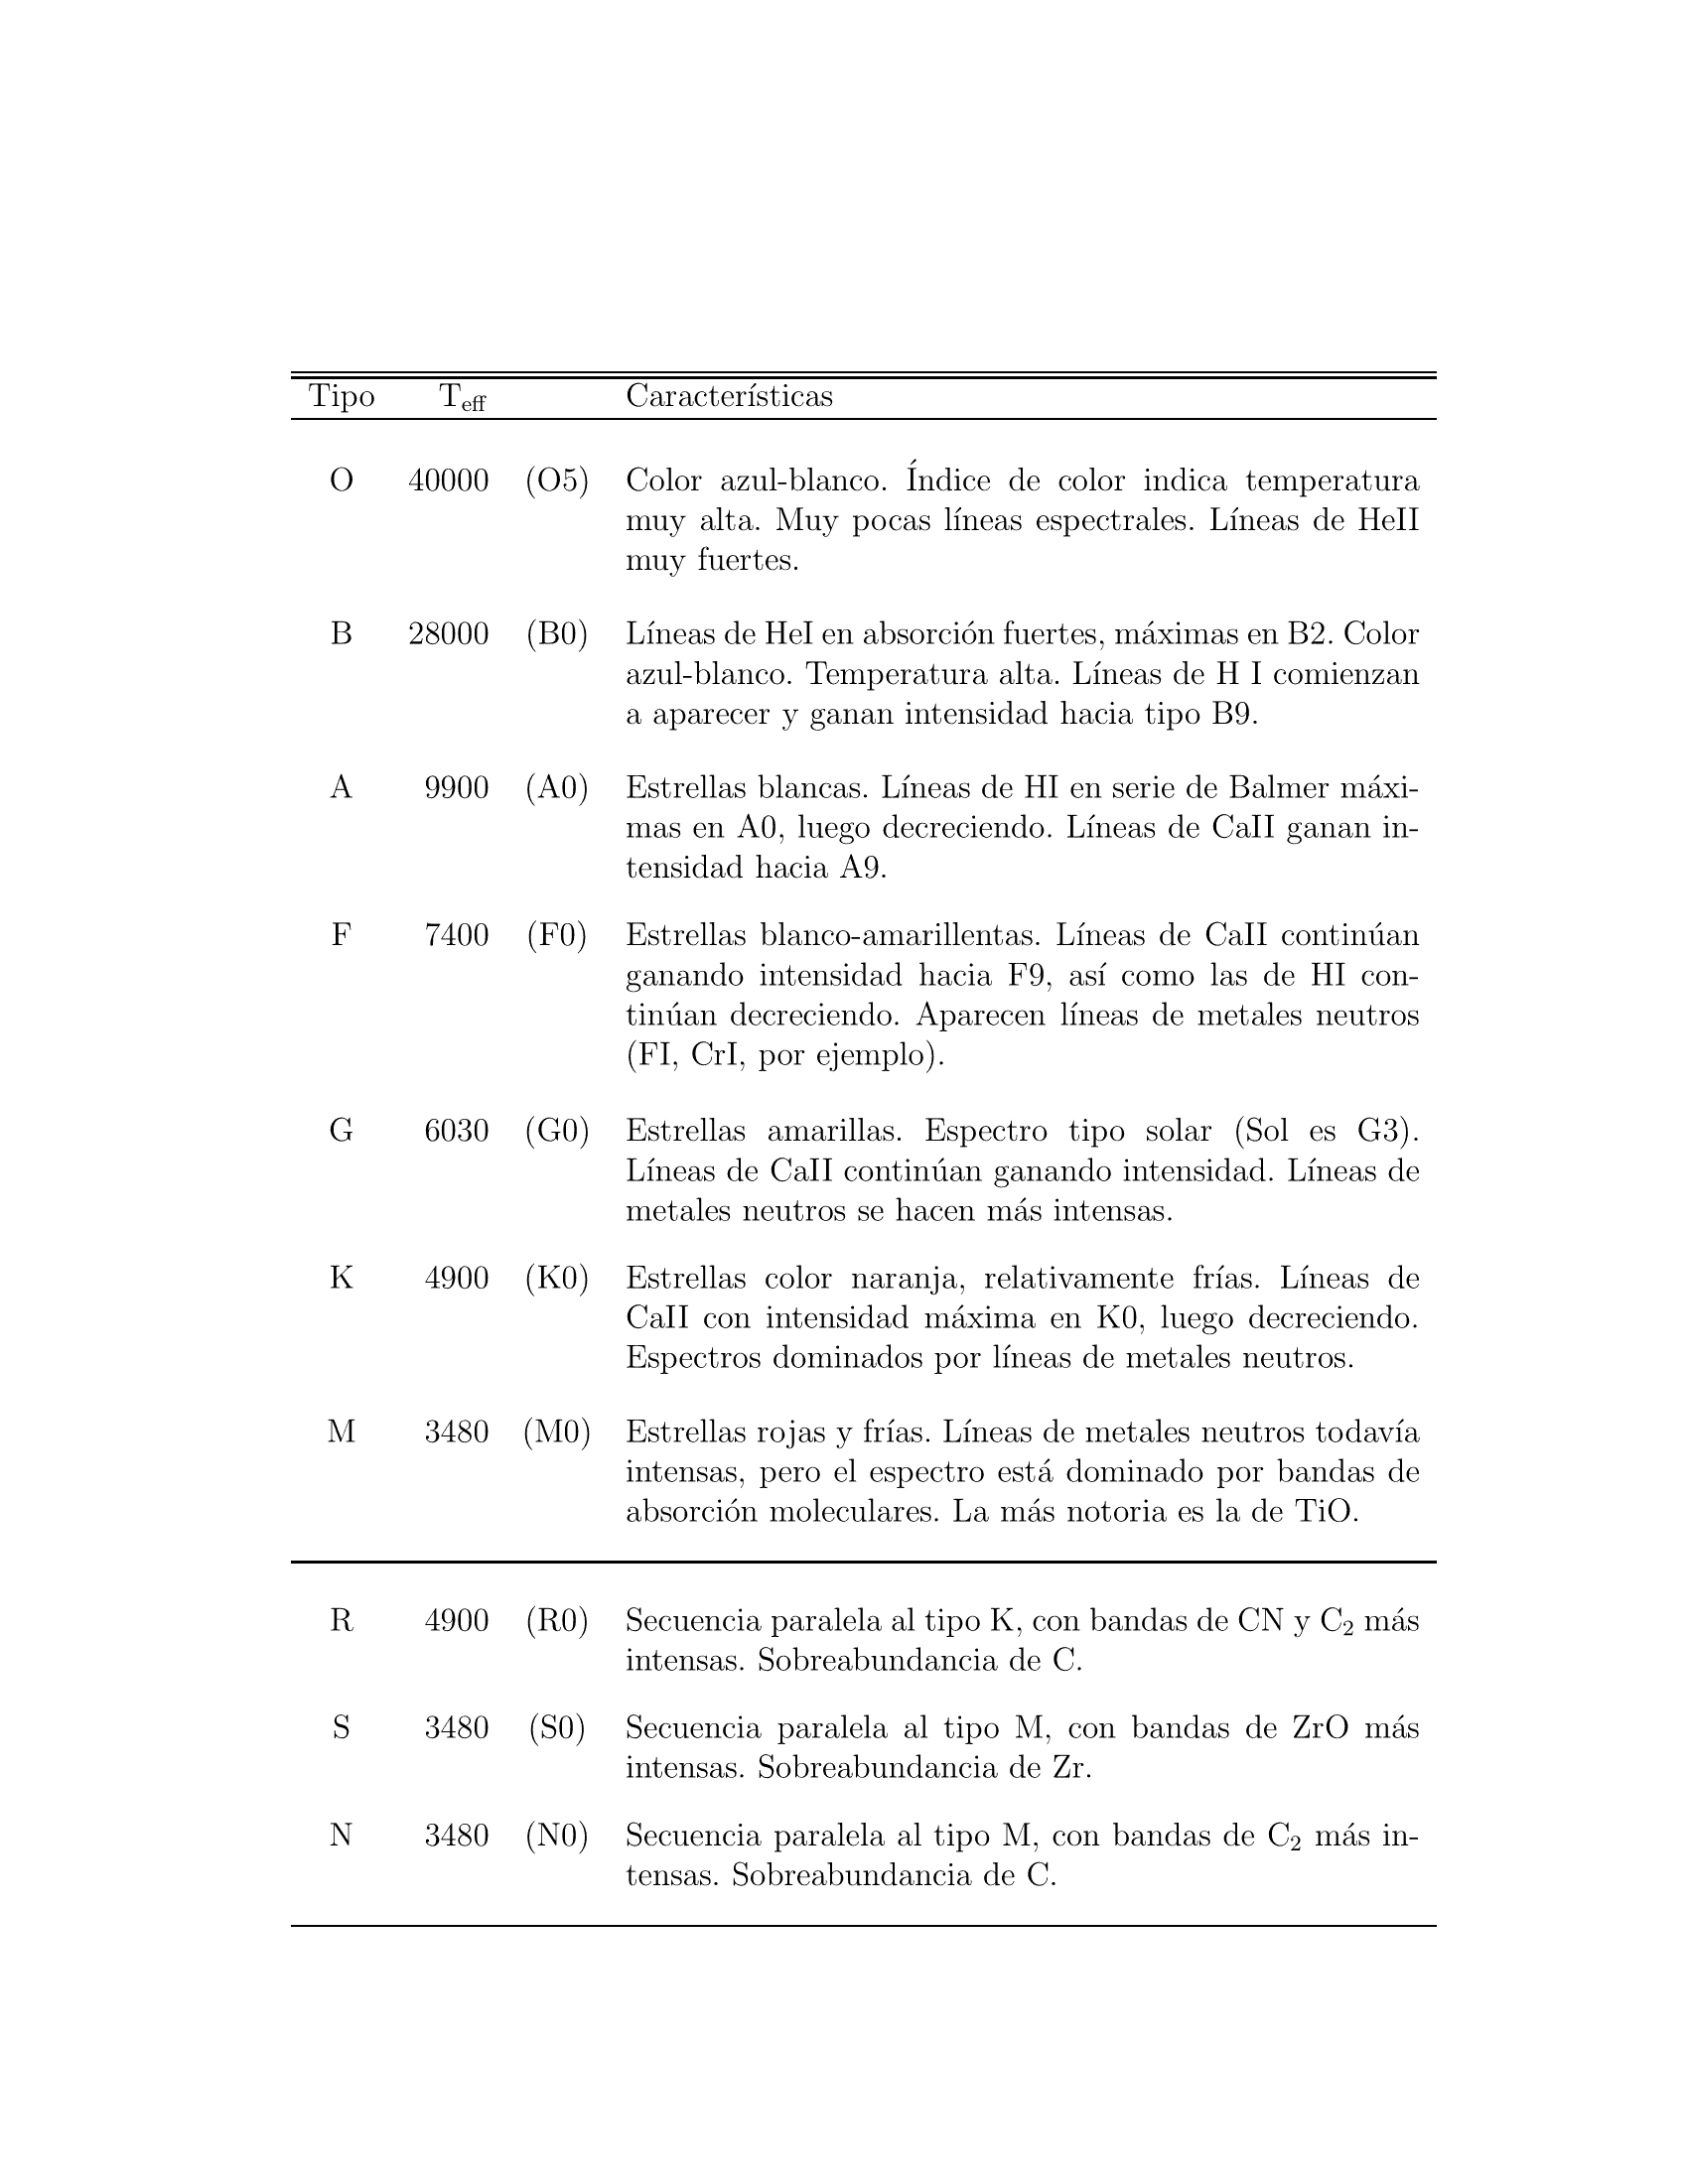
\includegraphics[width=0.85\textwidth]{tabla.png} 
\end{tabular}
\caption{{\small Tabla de algunas caracter'isticas para los distintos tipos espectrales extra'idas del libro ``Radiaci'on y Materia en Astrof'isica'' de Clocchiatti \& Catel'an (Tabla 7.1). En ella se pueden observar las distintas temperaturas para los distintos tipos espectrales. All'i tambi'en est'an los tipos R, S y N; clasificaciones que fueron originalmente consideradas por separado, pero en realidad son estrellas similar a las tipo K o M aunque con algunas l'ineas an'omalas/m'as intensas de lo esperado.}}\label{tabla}
\end{center} 
\end{figure}
\item Si observo una estrella cuya magnitud aparente en filtro $V$ es $m_V = -4$ y otra estrella cuya magnitud es $m_V = 2$. ?`Cu'al es m'as brillante y por qu'e? ?`C'omo se comparan sus luminosidades asumiendo que ambas estrellas tuviesen el mismo radio?

\vspace{2mm}

\emph{Sol:}

\vspace{2mm}

Cada vez que queramos comparar el brillo de dos objetos (ya sean galaxias, estrellas u otros) es importante recordar que dos magnitudes aparentes (brillo aparente) de un objeto se relacionan mediante la f'ormula:


\begin{equation} \label{mags_1}
m_1 - m_2 = -2.5 \log_{10} \bigg( \frac{F_1}{F_2} \bigg)
\end{equation}

donde $F_1$ es el flujo (energ'ia/'area/tiempo) de la estrella 1 cuya magnitud llamaremos para este ejercicio en espec'ifico $m_1 = -4$; y $F_2$ es el flujo para la estrella 2 cuya magnitud en este ejercicio ser'a $m_2 = 4$.

Aqu'i me extender'e un poco fuera del enunciado de la ayudant'ia para hacerles notar algunas cosas.

Primero, es com'un encontrar la ecuaci'on \eqref{mags_1} como:

\begin{equation} \label{mags_2}
m_1 - m_2 = 2.5 \log_{10} \bigg( \frac{F_2}{F_1} \bigg)
\end{equation}

en otras palabras, la ecuaci'on \eqref{mags_2} es exactamente a la ecuaci'on \eqref{mags_1}, pero se cambi'o la posici'on entre $F_1$ y $F_2$ en la divisi'on. Eso es porque no hay un s'imbolo ``-'' del lado derecho de la ecuaci'on. Lo que hace este s'imbolo ``-'' es simplemente cambiar de posici'on el denominador con el numerador en la ecuaci'on \eqref{mags_2} gracias a la propiedad de los logaritmos. Cabe notar que las ecuaciones \eqref{mags_1} y \eqref{mags_2} son completamente id'enticas. En mi caso personal, prefiero la ecuaci'on \eqref{mags_1} porque el $m_1$ va primero al lado izquierdo de la ecuaci'on y el $F_1$ va en la parte de arriba de la divisi'on al lado derecho de la ecuaci'on, pero si'entanse libres de usar cualquiera de las dos \emph{siempre y cuando no olviden el s'imbolo ``-'' cuando corresponde}. 

Otra cosa importante es que este logaritmo es en base 10. A veces los astr'onomos ``omiten'' anotar expl'icitamente el 10 y escriben ``$\log$'' solo, pero generalmente en astronom'ia se asume que el logaritmo ``por defecto'' es en base 10.

Adem'as, siempre es 'util recordar que existe una relaci'on entre la luminosidad y el flujo:

\begin{equation} \label{flujo-luminosidad}
\text{Luminosidad} = \text{Flujo} \times \text{'Area}
\end{equation}

Y de igual manera:

\begin{equation} \label{luminosidad-flujo}
\text{Flujo} = \frac{\text{Luminosidad}}{\text{'Area}}
\end{equation}

Si consideramos $F$ como flujo, $L$ como luminosidad y $\text{'Area} = 4 \pi R^2$ como el 'area superficial de una esfera (donde $R$ es el radio del objeto, en este caso la estrella) la ecuaci'on \eqref{luminosidad-flujo} es simplemente:

\begin{equation} \label{F_L}
F = \frac{L}{4 \pi R^2}
\end{equation}

Ahora, para una estrella 1 (con magnitud $m_1$, flujo $F_1$, luminosidad $L_1$ y radio $R_1$) y una estrella 2 (con magnitud $m_2$, flujo $F_2$, luminosidad $L_2$ y radio $R_2$) tendremos que si utilizamos la ecuaci'on \eqref{F_L} en \eqref{mags_1} obtenemos:

\begin{equation*}
m_1 - m_2 = -2.5 \log_{10} \bigg(\frac{\frac{L_1}{4 \pi R_1^2}}{\frac{L_2}{4 \pi R_2^2}} \bigg) = -2.5 \log_{10} \bigg(\frac{L_1}{R_1^2} \cdot \frac{R_2^2}{L_2} \bigg)
\end{equation*}

Es decir,

\begin{equation} \label{luminosidad_magnitud}
m_1 - m_2 = -2.5 \log_{10} \bigg( \frac{L_1}{L_2} \times \bigg[\frac{R_2}{R_1} \bigg]^2 \bigg)
\end{equation}

Finalmente, podemos establecer una relaci'on entre las magnitudes de dos objetos y sus temperaturas efectivas.

Recordemos que existe una relaci'on entre el flujo y la temperatura dada por la proporci'on:

\begin{equation}
\text{Flujo} \ \propto \ \text{Temperatura}^4
\end{equation}

M'as en espec'ifico, ambas se relacionan con la conocida Ley de Stefan-Boltzmann:

\begin{equation} \label{stefan-boltzmann}
F = \sigma T_{\rm eff}^4
\end{equation}

donde $F$ es el flujo, $\sigma$ es la constante de Stefan-Boltzmann cuyo valor es $\sigma = 5.67 \times 10^{-8} \ W \cdot m^{-2} \cdot K^{-4}$; y $T_{\rm eff}$ es la temperatura efectiva (es decir, la temperatura absoluta -que se mide en Kelvin- de la superficie).

De manera que para una estrella 1 (con magnitud $m_1$ y temperatura efectiva $T_{\rm eff,1}$) y una estrella 2 (con magnitud $m_2$ y temperatura efectiva $T_{\rm eff,2}$) tenemos, al utilizar la ecuaci'on \eqref{stefan-boltzmann} en \eqref{mags_1}, la relaci'on:

\begin{equation*}
m_1 - m_2 = -2.5 \log_{10} \bigg( \frac{\sigma T_{\rm eff,1}^4}{\sigma T_{\rm eff,2}^4} \bigg) = -2.5 \log_{10} \bigg( \frac{T_{\rm eff,1}}{T_{\rm eff,2}} \bigg)^4 = -10 \log_{10} \bigg( \frac{\sigma T_{\rm eff,1}}{\sigma T_{\rm eff,2}} \bigg)
\end{equation*}

De manera que podemos hallar una relaci'on aproximada entre las temperaturas de dos objetos:

\begin{equation}
\frac{T_{\rm eff,1}}{T_{\rm eff,2}} = 10^{([m_2 - m_1]/10)} 
\end{equation}

Finalmente, podemos relacionar la temperatura con la luminosidad de una estrella mediante las ecuaciones \eqref{F_L} y \eqref{stefan-boltzmann}. 

\begin{equation}
F = \sigma T_{\rm eff}^4 = \frac{L}{4 \pi R^2}
\end{equation}

Con esto se podr'ia, por ejemplo, estimar la temperatura efectiva de una estrella mediante:

\begin{equation}
T_{\rm eff} = \frac{1}{\sqrt{R}} \bigg( \frac{L}{4 \pi \sigma} \bigg)^{1/4}
\end{equation}

Ahora bien, estas relaciones son aproximadas dado que, por ejemplo, hay veces que entre el astro y nosotros puede existir polvo. Este polvo puede absorber o dispersar la luz. Adem'as est'a el gran problema de que la absorci'on y dispersi'on afectan m'as a los colores azules que a los rojos (es decir, afecta m'as a estrellas de mayores temperaturas que de menores temperaturas). De manera que, recalco, esta relaci'on solo sirve para tener una noci'on de c'omo se relacionan las temperaturas de dos objetos y no es del todo exacta.
  
\vspace{2mm}

Toooodo lo anterior lo hice para que se den cuenta de que pueden ``jugar'' con las ecuaciones para ir despejando aquello que vayan necesitando mediante distintas relaciones que ya han visto en clases.

\emph{Volviendo al problema original}, el cual es comparar dos estrellas; la estrella 1 con magnitud $m_1 = -4$ y estrella 2 con magnitud $m_2 = 2$, nos piden comparar sus luminosidades. Como nos piden comparar las luminosidades y lo 'unico que conocemos de las estrellas es su magnitud, la ecuaci'on ``ideal'' que hallamos para resolver este problema es la ecuaci'on \eqref{luminosidad_magnitud}; la cual anoto aqu'i por comodidad:

\begin{equation*} 
m_1 - m_2 = -2.5 \log_{10} \bigg( \frac{L_1}{L_2} \times \bigg[\frac{R_2}{R_1} \bigg]^2 \bigg)
\end{equation*}

Reemplazando por los valores correspondientes simplemente y recordando que en este caso se dice que ambas estrellas tienen un radio similar (es decir, $R_1 \approx R_2$) hallamos:

\begin{equation*}
-4 - (+2) = -2.5 \log_{10} \bigg( \frac{L_1}{L_2} \times \cancelto{1}{\bigg[\frac{R_2}{R_1} \bigg]^2} \bigg)
\end{equation*}

Dando as'i:

\begin{equation*}
-6 = -2.5 \log_{10} \bigg(\frac{L_1}{L_2} \bigg)
\end{equation*}

Desarrollando:

\begin{equation*}
\frac{6}{1} \cdot \frac{2}{5} = \log_{10} \bigg(\frac{L_1}{L_2} \bigg)
\end{equation*}

Dando as'i:

\begin{equation*}
10^{12/5} = \frac{L_1}{L_2}
\end{equation*}

Finalmente obtenemos:

\begin{equation}
L_1 \approx 250 L_2
\end{equation}

Es decir, la estrella 1 es aparentemente unas 250 veces m'as luminosa que la estrella 2. Si $m_1 = -4$ y $m_2 = 2$, ?`tiene esto sentido? Recordemos que las magnitudes se relacionan con los brillos, pero son ``anti intuitivos''. Mientras menor sea una magnitud, mayor es el brillo. De manera que s'i tiene sentido que $L_1 > L_2$ si $m_1 < m_2$.

\item En astronom'ia generalmente se define el color como la resta de la magnitud medida para un mismo objeto en dos filtros distintos. Por ejemplo: medimos la magnitud de una estrella en filtro ``$B$'' 'esta nos da una magnitud de $m_B = 3.8$ y al medir la magnitud en filtro ``$V$'' 'esta nos da $m_V = 4.0$. Por convenci'on, siempre se resta el filtro m'as rojo al filtro m'as azul; por ejemplo, en este caso, tendr'iamos $B-V = -0.02$. ?`Qu'e se puede inferir entonces de una estrella si medimos su magnitud en 2 filtros distintos?

\vspace{2mm}

\emph{Sol:}

\vspace{2mm}

Los filtros en astronom'ia sirven para capturar (m'as) fotones de una cierta/frecuencia longitud de onda. Recordemos que una fuente de luz puede estar emitiendo en todo el espectro electromagnético, pero de tooodo el espectro hay ciertas longitudes de ondas espec'ificas que nos interesan para distintos prop'ositos. Por ejemplo, est'a el filtro $B$ (Blue) y $V$ (Visual). Con el primero obtenemos fotones m'as azules y con el segundo fotones m'as cercanos al color verde. Entonces, se mide la magnitud en 2 filtros distintos para una misma estrella y 'estas mediciones se restan la una de la otra. De esta manera lo que se halla para una estrella o galaxia es su \emph{color}. De manera que tendremos, de la manera m'as general para un mismo objeto:

\begin{equation}
\text{Magnitud en filtro m'as azul} - \text{Magnitud en filtro m'as rojo} = \text{Color}
\end{equation}

Y como ya hemos visto, el color de una estrella nos dice muchas cosas: como su \emph{temperatura}.

De manera que el \emph{color se relaciona altamente con la temperatura de una estrella}.

\item ¿Qu'e es un diagrama Hertzprung-Russel, tambi'en conocido como diagrama H-R o diagrama Color-Magnitud, y por qu'e es tan utilizado en astronom'ia?

\vspace{2mm}

\emph{Sol:}

\vspace{2mm}

El diagrama HR es un diagrama que relaciona las luminosidades (o magnitudes absolutas) de las estrellas con su temperatura (o colores). Por lo mismo, tambi'en es com'un hallar este diagrama por el nombre Diagrama Color-Magnitud. Este diagrama es sumamente 'util para el estudio de poblaciones estelares. Un ejemplo de lo que representa puede ser hallado en la Figura \ref{hr_diagr}.

\begin{figure}[!ht]
\begin{center}
\begin{tabular}{ll}
  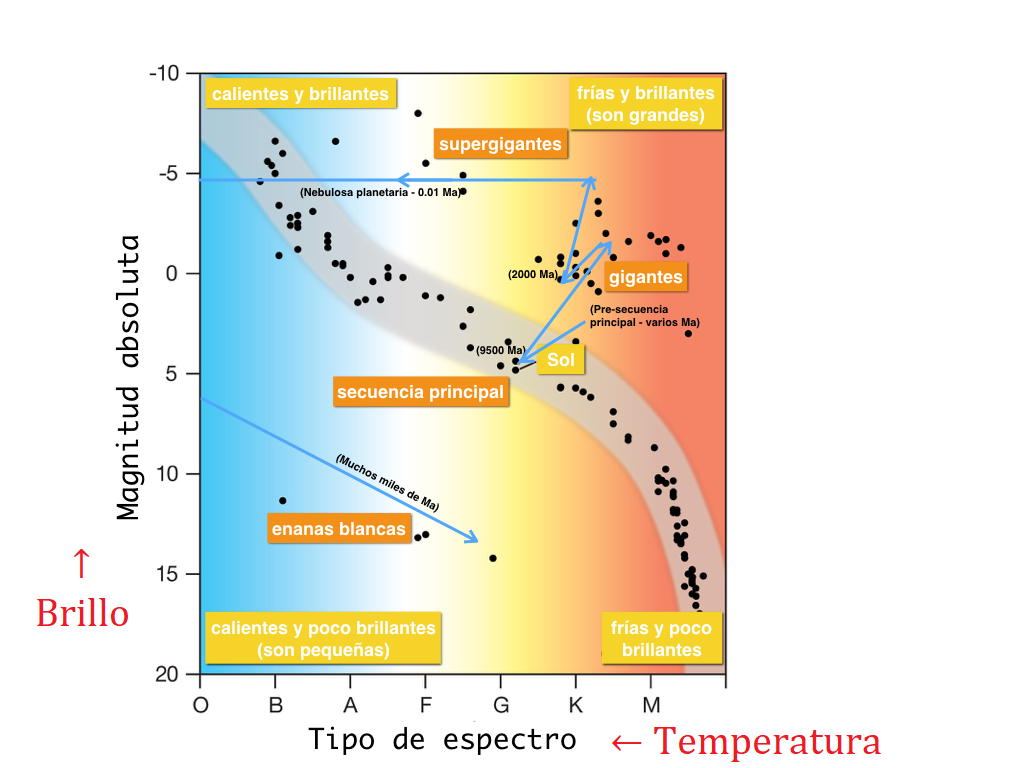
\includegraphics[width=0.85\textwidth]{diagrama_hr.png} 
\end{tabular}
\caption{{\small Diagrama HR. Note que una cosa importante de este diagrama es que es b'asicamente un diagrama de brillo (luminosidad/magnitud absoluta) vs. temperatura. El brillo crece de abajo hacia arriba en el eje Y, \emph{pero} la temperatura crece de derecha a izquierda en el eje X. La figura muestra, adem'as, las distintas fases por las que una estrella puede pasar a lo largo de su vida.}}\label{hr_diagr}
\end{center} 
\end{figure}

Por ejemplo, en un diagrama HR podemos medir la edad aproximada de un c'umulo globular; recuerden que un c'umulo globular es un grupo de estrellas muy juntas entre s'i y que se mueven como una ``manada'' gracias a la gravedad que las tiene atada entre ellas (ver Figura \ref{hr}(a)). Por ejemplo, para construir un diagrama Color-Magnitud para un c'umulo globular lo que se hace en general es lo siguiente (aunque en realidad es un poco m'as complejo):

\begin{enumerate} [i)]
\item Para cada estrella en el campo de visi'on del c'umulo globular se mide su magnitud en distintos filtros. Deben ser m'inimo en 2 filtros distintos para realizar un diagrama Color-Magnitud, de otra manera no se puede obtener su color. Por ejemplo, supongamos que tenemos que medir la magnitud de una estrella en el filtro $B$ y $V$ para obtener su color.

\item Una vez medida las magnitudes en distintos filtros para las estrellas que est'an en el campo de visi'on, se realiza un gr'afico donde en el eje X va el color; es decir, el eje X representa $B-V$ en nuestro ejemplo.

\item En el eje Y se pone la magnitud medida en un solo filtro; puede ser cualquiera de las magnitudes medidas en uno de los filtros. En este ejemplo en concreto, elijamos el eje Y como magnitud $V$.

\item Ahora se ponen los datos medidos para cada estrella en el diagrama. Por ejemplo, supongamos que realizamos un diagrama Color-Magnitud donde en el eje Y tenemos la magnitud $V$ y en el eje X tenemos el color $B-V$. Para \textit{una sola estrella} supongamos que medimos una magnitud de $m_V = V = 6.0$ y $m_B = B = 6.2$. De manera que tendremos que el color de esta estrella en este diagrama es $B-V = 6.2 - 6.0 = 0.2$. De esta manera, las coordenadas de esta estrella en nuestro diagrama ser'an $[B-V, \ V] = [0.2, \ 6.0]$.

\item Se repite el paso anterior, pero esta vez para \emph{todas las estrellas} del c'umulo globular (el paso anterior era s'olo para una estrella).

\item El resultado es un diagrama como el mostrado en la Figura \ref{hr} (abajo). Cada punto all'i es una estrella. En general uno encuentra que las estrellas siguen un camino desde la parte inferior derecha, cruzan en diagonal y, de la nada, se dan una vuelta. Todas estas secciones (la parte donde las estrellas se encuentran en el camino ``diagonal'' o donde se dan una vuelta) tienen mucho que ver con evoluci'on estelar.
\end{enumerate}

\begin{figure} [h!]
\centering
\begin{subfigure}[b]{0.5\textwidth}
   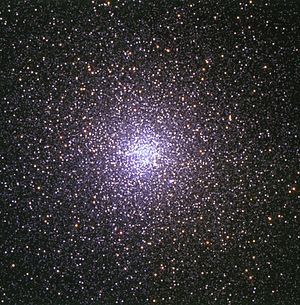
\includegraphics[width=1\linewidth]{47_tuc.jpg}
   \caption{Foto del c'umulo globular 47 Tuc (o tambi'en llamado NGC 104).}
   \label{fig:Ng1} 
\end{subfigure}

\begin{subfigure}[b]{0.7\textwidth}
   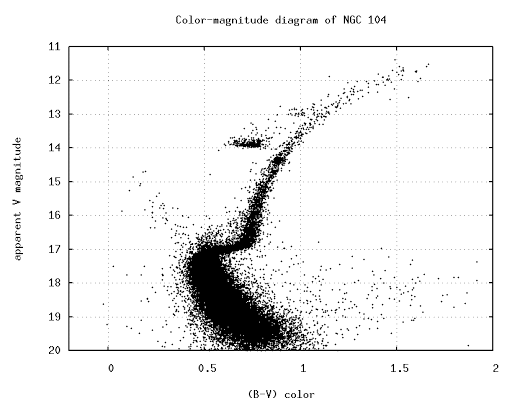
\includegraphics[width=1\linewidth]{cmd_ngc_104.png}
   \caption{Diagrama Color-Magnitud para NGC 104}
   \label{fig:Ng2}
\end{subfigure}
\caption{Obtenci'on de un diagrama Color-Magnitud. Note algo importante: Cada uno de los puntos del gr'afico abajo es apenas una estrella de todas de las que est'an en la imagen superior.}
\label{hr}
\end{figure}

De manera que, en general, los c'umulos globulares son excelentes laboratorios estelares. Porque tienen dos ventajas: i) Tienen muchas estrellas (lo que es una muestra grande y estad'isticamente da m'as seguridad). ii) Al ser tantas estrellas, es muy probable que encontremos estrellas en cada una de las distintas fases estelares (puesto que hay algunas fases estelares ``fugaces'' y cuesta hallar estrellas de ese tipo para estudiarlas), lo que nos permite su estudio.
\end{enumerate}

\newpage
\begin{tiny}
.

.

.
\end{tiny}


\textbf{Problema 2. Estrellas de baja masa vs. estrellas de alta masa}

\vspace{3mm}


\begin{enumerate}[a)]
\item ?`Cu'ales son los rangos (aproximados\footnote{Digo ``aproximados'' porque en la literatura siempre encontrar'a valores \emph{similares}, pero \emph{no necesariamente iguales}. No hay una definici'on 'unica.}) para las estrellas de baja, intermedia y alta masa?

\vspace{2mm}
\emph{Sol:}
\vspace{2mm}

Uno de los par'ametros m'as importantes de las estrellas es su masa ($M$). Ella nos va a decir, entre muchas cosas, c'omo es que va a evolucionar esta estrella.

Si bien los rangos son variables, en general es bastante aceptable que los rangos para masas est'en dados por:

\begin{equation*}
M < 2.2 \ M_\odot \ \ \ \ \ \ \ \ \ \ \ \ \text{Baja masa}
\end{equation*}

\begin{equation*}
 2.2 \ M_\odot < M < 8 \ M_\odot \ \ \ \ \ \ \ \ \ \text{Masa intermedia}
\end{equation*}

\begin{equation*}
M > 8 \ M_\odot \ \ \ \ \ \ \ \ \ \ \ \ \ \ \ \text{Alta masa}
\end{equation*}



\item De los rangos anteriores en base a la masa, ?`cu'ales esperar'ia que fuesen las estrellas que m'as o menos viven y por qu'e?

\vspace{2mm}
\emph{Sol:}
\vspace{2mm}

La luminosidad $L$ de una estrella escala con su masa $M$ de la siguiente manera:

\begin{equation}
L \ \propto \ M^{3}
\end{equation}

(aunque, en realidad, escala aproximadamente como $L \ \propto \ M^{3.5}$)

De cierta manera, podemos ver la luminosidad como una especie de ratio al cual la estrella est'a liberando energ'ia por unidad de tiempo: mientras m'as est'e quemando m'as luminosa ser'a (aunque hay un l'imite para la luminosidad que una estrella puede alcanzar sin ``romperse'', llamado el l'imite de Eddington).

La relaci'on entre el tiempo de vida $\tau$ y su masa est'a dada aproximadamente por:

\begin{equation}
\tau \ \propto \ M^{-2.5}
\end{equation}

Es decir, mientras m'as masa tenga una estrella, menos vive 'esta.

?`Por qu'e se puede deber esto? Es decir, si tenemos m'as masa para una estrella m'as masiva ello quiere decir que tiene m'as combustible disponible para quemar y, por ende, uno tender'ia a creer que esta estrella vivir'ia m'as. El problema yace en la luminosidad. Como la luminosidad es la cantidad de energ'ia que emite por unidad de tiempo, si nos fijamos bien la luminosidad escala en un factor alto con la masa, tan alto que incluso aunque la estrella masiva tenga m'as combustible para quemar ello no implica que la estrella vivir'a m'as. A modo de ejemplo, comparemos una estrella muy masiva de $10 \ M_\odot$ con otra poco masiva como el Sol (de $1 \ M_\odot$). La estrella masiva tiene 10 veces m'as combustible para quemar y transformar en energ'ia que el Sol. Sin embargo, esta estrella emite 1000 veces m'as energ'ia que el Sol. La estrella masiva emite 1000 veces m'as, pero s'olo tiene 10 veces m'as masa que el Sol. Ello quiere decir entonces que esta estrella vivir'a al menos $1000/10 \approx 100$ veces menos que el Sol.

\vspace{2mm}

Ello implica entonces que las estrellas muy masivas viven poco en comparaci'on con sus compa'neros de baja masa. Por lo mismo, las estrellas masivas son ``raras'' de encontrar por dos razones:

\begin{enumerate} [i)]
\item Viven menos, ``solo'' unas decenas a cientos millones de a'nos\footnote{Si bien decenas o cientos de millones de a'nos puede parecer much'isimo, en escala astron'omica para edad de estrellas esto no es tanto tiempo.}.

\item Es m'as com'un que en el universo se formen estrellas de baja masa que de alta masa.
\end{enumerate}

De manera que las estrellas de alta masa son raras porque cuesta que se formen y, de las pocas que se forman, viven muy poco. Por lo que hallar una estrella muy masiva es, realmente, una aguja en un pajar. Adem'as, son bastante caracter'isticas porque son muy azules dada su alta temperatura.

De la misma manera, las estrellas m'as viejas y comunes en el universo son las estrellas no muy masivas (baja masa) $\sim 0.6-0.8 \ M_\odot$ ya que pasa totalmente lo contrario a las estrellas masivas: viven mucho y se forman muchas.


\item ?`Se espera que una estrella de alta masa sea m'as o menos luminosa que una estrella como el Sol? ?`Y qu'e es lo que se espera para el tiempo de vida de una estrella masiva con respecto a una estrella no masiva? Compare sus respuestas de la luminosidad y tiempo de vida que se espera para una estrella de $1 \ M_\odot$ con otra de $10 \ M_\odot$. ?`Qu'e puede inferir de estos resultados? Dato (quiz'as) 'util: %Asuma que la luminosidad del Sol es $L \sim 4 \times 10^{26} \ \text{W}$ y su tiempo de vida es $\tau_\odot \approx 10^{10} \ \text{yr}$.
tiempo de vida del Sol est'a estimado en $\tau_\odot \approx 10^{10} \ \text{yr}$.

\vspace{2mm}
\emph{Sol:}
\vspace{2mm}

(Las respuestas a las dos primeras  preguntas de este 'item fueron respondidas en el 'item anterior).

Ya que queremos comparar el tiempo de vida\footnote{En realidad este ``tiempo de vida'' es el tiempo en el que las estrellas pasan en la fase de Secuencia Principal, fase evolutiva de las estrellas donde queman hidr'ogeno en el n'ucleo. Sin embargo, las estrellas pasan casi la totalidad de su vida ($\sim 90\%$) en esta fase evolutiva. Por lo que considerar el tiempo de una estrella en Secuencia Principal como su tiempo de vida no es del todo descabellado.} para una estrella de $10 \ M_\odot$ con el tiempo de vida del Sol, y sabemos que: $\tau \ \propto \ M^{-2.5}$. De manera que simplemente comparamos:

\begin{equation}
\frac{\tau}{\tau_\odot} \sim \bigg( \frac{M}{M_\odot} \bigg)^{-2.5}
\end{equation}

donde $\tau$ es el tiempo de vida (en Secuencia Principal) de la estrella que queremos compara y $M$ es la masa de dicha estrella a comparar.

De manera que, despejando:

\begin{equation}
\tau \sim \tau_\odot \bigg( \frac{M}{M_\odot} \bigg)^{-2.5}
\end{equation}

Reemplazando por los valores dados en el enunciado:

\begin{equation*}
\tau \sim (10^{10} \ \text{yr}) \times \bigg( \frac{10 \ M_\odot}{M_\odot} \bigg)^{-2.5} \sim  10^{10}  \times 3 \times 10^{-3} \ \text{yr} \sim = 3 \times 10^{7} \ \text{yr} = 30 \ \text{Myr}
\end{equation*}

Es decir, una estrella 10 veces m'as masivas que el Sol vivir'a unas 300 veces menos.

(La discrepancia entre este ejercicio y el ejemplo que d'i en el item anterior, donde dec'ia que una estrella de $10 \ M_\odot$ vive 100 veces menos, era porque antes consideramos 
$L \ \propto \ M^{3}$; mientras que en este item consideramos impl'icitamente $L \ \propto \ M^{3.5}$. Aunque ambas respuestas nos dan dentro del mismo orden de magnitud [de decenas de millones de a'nos]).
\item Hasta donde sabemos, el Sol est'a constantemente fusionando hidr'ogeno en su n'ucleo cuando 'este se encuentra en la fase de Secuencia principal (o en ingl'es, Main-Sequence [MS]). Sin embargo, el proceso a trav'es del cual el hidr'ogeno es ``quemado'' dentro del n'ucleo de las estrellas es distinto. 

Para estrellas en MS, ?`en qu'e se diferencia la quema de hidr'ogeno para una estrella de baja masa con una de alta masa?

\newpage

\begin{figure}
\centering
  \begin{subfigure}{6cm}
    \centering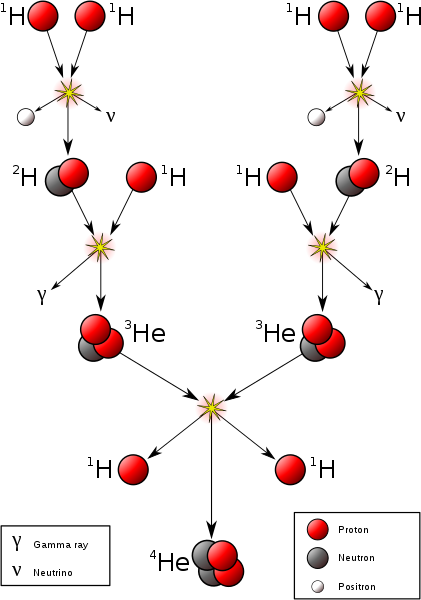
\includegraphics[width=6cm]{p-p.png}
    \caption{Cadena prot'on-prot'on}
  \end{subfigure}
  \begin{subfigure}{6cm}
    \centering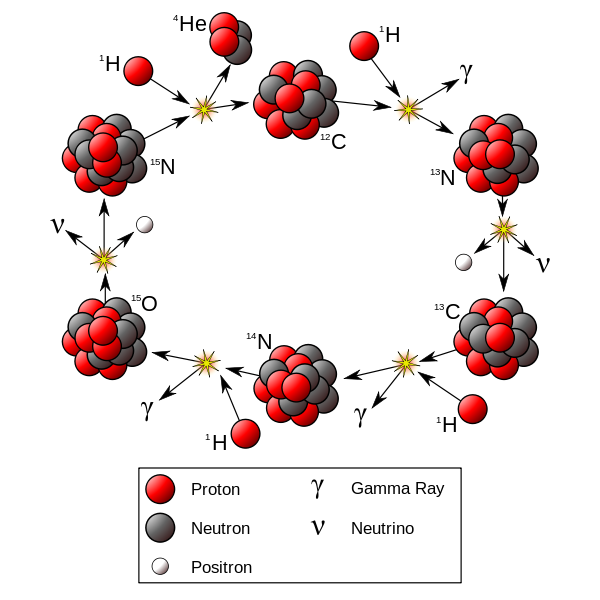
\includegraphics[width=8.5cm]{cno.png}
    \caption{Ciclo CNO}
  \end{subfigure}
  \caption{Distintas reacciones de fusi'on que se pueden generar dentro de una estrella. Cu'al es la que va a dominar depende de la masa de la estrella.}
\end{figure} 
\vspace{3mm}



\vspace{2mm}
\emph{Sol:}
\vspace{2mm}
?`Alguna vez se han preguntado c'omo es que el Sol genera ese calor tan intenso que nos llega? Y la respuesta es simple, pero compleja a la vez: fusi'on nuclear.

La fusi'on nuclear consiste en el proceso donde n'ucleos at'omicos de carga similar se unen y producen un elemento m'as pesado, adem'as de energ'ia. Es decir, a modo muy simplificado, la fusi'on nuclear se puede ver c'omo:

\begin{equation}
\text{Elemento liviano 1} + \text{Elemento liviano 2} \rightarrow \text{Elemento m'as pesado} + \text{Energ'ia}
\end{equation}

Se diferencia de la fisi'on nuclear, la cual es que ocurren en las plantas nucleares aqu'i en la Tierra. La fisi'on nuclear es al rev'es; de un elemento muy pesado se generan otros m'as livianos, m'as energ'ia. A modo muy simple, la fisi'on puede verse como:

\begin{equation}
\text{Elemento m'as pesado} \rightarrow \text{Elementos m'as livianos} + \text{Energ'ia}
\end{equation}

La fusi'on nuclear ocurre en el Sol. En la Tierra no se ha podido lograr dada sus extremas condiciones: se requieren densidades muy altas, de unos $150 \ \text{gr} \cdot \text{cm}^{-3}$ (unas 8 veces m'as denso que el oro) y una temperatura de $T = 15 \times 10^{6} \ \text{K}$; condiciones demasiado extremas para ser replicadas, sin que decaigan con el tiempo, en un laboratorio. 

Lo que ocurre es que el ambiente es tan denso y tan caliente que los 'atomos de hidr'ogeno ionizados (que no son m'as que un prot'on) chocan unos con otros con tal velocidad y momentum que quedan ``pegados'', formando elementos m'as pesados y liberando energ'ia al sistema. Ahora bien, existen dos ``mecanismos'' de fusi'on nuclear del hidr'ogeno: la cadena prot'on-prot'on (p-p chain) y el Ciclo CNO (CNO Cycle). Si bien no entrar'e en detalle de las distintas fases de estas cadenas (que es algo que ver'an m'as adelante en detalle en Astrof'isica Estelar), de manera muy vaga ambas cadenas pueden ser descritas de la siguiente manera:

\begin{enumerate} [i)]

\item Cadena p-p:

\begin{equation} \label{p-p_chain}
4 \ \text{p} \rightarrow \text{Muchos procesos} \rightarrow 1 \ \text{He} + \text{Energ'ia}
\end{equation}

(Notar que un hidr'ogeno ionizado es lo mismo que un prot'on, es decir $1 \ \text{H}^+ = 1\ \text{p}$).

\textit{En resumen, se comienza con 4 protones y se termina con un 'atomo de Helio m'as energ'ia.}

\item Ciclo CNO:


\begin{equation} \label{CNO_cycle}
^{12}\text{C} + \text{p} \rightarrow \text{Procesos que incluyen N y O} \rightarrow ^{12}\text{C} + \text{He} + \text{Energ'ia}
\end{equation}

\begin{center}
{\Huge $\circlearrowright$}
\end{center}
\end{enumerate}

Notemos algo muy importante: en el ciclo CNO se comienza con un 'atomo de carbono y un prot'on -donde el 12 indica el n'umero m'asico (protones $+$ neutrones en el n'ucleo)- y el proceso termina con el mismo 'atomo de carbono, un 'atomo de Helio y energ'ia liberada. Se llama ``ciclo'' porque uno de los reactantes (el $^{12}\text{C}$), luego de pasar por toda la cadena, termina como producto de la reacci'on. El carbono se ``recicla'' (de all'i la palabra ``ciclo'') y as'i empieza el c'irculo para terminar formando un nuevo 'atomo de helio a partir de un n'ucleo de hidr'ogeno y carbono reciclado; el 'atomo de carbono vuelve a reaccionar con otro prot'on y as'i...

\vspace{2mm}

Ahora bien, ?`cu'al es el que domina en las estrellas? La respuesta, nuevamente, yace en la masa de las estrellas. Mientras m'as masiva sea una estrella mayores temperaturas y densidades se alcanzan en su interior. Este ambiente ``favorable'' hace que el Ciclo CNO domine en estrellas de alta masa. Por otro lado, para estrellas no masivas como el Sol, las condiciones son favorables para que la cadena p-p predomine. De manera que las reacciones nucleares en nuestro Sol son principalmente a trav'es de la cadena p-p.

Algo importante de mencionar es que estos dos caminos que puede tomar la fusi'on nuclear dentro del n'ucleo de una estrella \emph{no son excluyentes}. Es decir, ambos ocurren al mismo tiempo. \emph{Lo 'unico que dictar'a la masa de una estrella ser'a cu'al de las dos reacciones es la que domina, pero ambas ocurren a la vez en el n'ucleo de una estrella en distinta proporci'on}.
\end{enumerate}

\begin{figure}[!ht]
\begin{center}
\begin{tabular}{ll}
  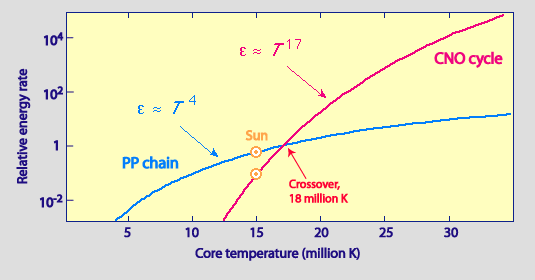
\includegraphics[width=0.9\textwidth]{comparison.png} 
\end{tabular}
\caption{{\small Ratio de energ'ia (por distintas reacciones de fusi'on nuclear) vs temperatura del n'ucleo en estrellas. Se puede ver que para menores temperaturas internas (estrellas de baja masa) la cadena p-p es la que predomina, pero a medida que nos vamos a temperaturas del n'ucleo m'as altas (estrellas m'as masivas) el ciclo CNO empieza a ganar peso y dominar por sobre la cadena p-p.}}\label{comparison}
\end{center} 
\end{figure}

\newpage

\textbf{Problema 3. El Sol}

\vspace{3mm}


Considere una estrella como el Sol, con una masa de aproximadamente $M_\odot \approx 2 \times 10^{30} \ \text{kg}$ y una luminosidad de aproximadamente $L \sim 4 \times 10^{26} \ \text{W}$, con $\text{W} = \text{kg} \ \text{m}^2/\text{s}^3$. Por simplicidad, asuma que el Sol estaba
compuesto por hidrógeno y nada m'as al momento de su formaci'on. Considere que el Sol emite energ'ia
transformando núcleos de hidrógeno (con masa dada por $m_{\rm H} = 1.67 \times 10^{-27} \ \text{kg}$) en núcleos de helio ($m_{\rm He} = 6.65 \times 10^{-27} \ \text{kg}$).

\begin{enumerate} [a)]
\item ?`Cu'antos 'atomos de hidr'ogeno se necesitan para crear un 'atomo de helio?

\vspace{2mm}
\emph{Sol:}
\vspace{2mm}

Basados en el Problema anterior, m'as en espec'ifico en la reacci'on \eqref{p-p_chain}, se puede decir que la base de la cadena p-p es que empezamos con 4 protones y terminamos con un 'atomo de helio m'as energ'ia. De manera que necesitamos 4 n'ucleos de hidr'ogeno para formar uno de helio.

\item ?`Cu'al es, aproximadamente, la diferencia porcentual de masa entre los ingredientes y los productos de la reacci'on nuclear para el Sol? ?`Es la diferencia positiva o negativa? ?`Qu'e implica aquello?

\vspace{2mm}
\emph{Sol:}
\vspace{2mm}

La masa de un 'atomo de hidr'ogeno\footnote{La masa de un 'atomo de hidr'ogeno es pr'acticamente la misma que la masa de un prot'on. Esto porque para un 'atomo de hidr'ogeno, conformado por un electr'on y un prot'on, la masa del electr'on es unas 1000 veces m'as pequeña que la del prot'on. Por lo que $m_{\rm H} = m_{\rm p} + m_{\rm e} \approx m_{\rm p}$, ya que $m_{\rm p} \gg m_{\rm e}$.} es de $m_{\rm H} = 1.67 \times 10^{-27} \ \text{kg}$. Como necesitamos 4 n'ucleos de hidr'ogeno para formar uno de helio, primero calculamos la masa de 4 n'ucleos de hidr'ogeno:

\begin{equation}
4 \times m_{\rm H} = 4 \times 1.67 \times 10^{-27} \ \text{kg} \approx 6.68 \times 10^{-27} \ \text{kg}
\end{equation}

Por otra parte, la masa de un 'atomo de helio es:

\begin{equation}
m_{\rm He}  = 6.65 \times 10^{-27} \ \text{kg}
\end{equation}

Comparando las masas de ambos elementos, llegamos a:

\begin{equation}
\frac{m_{\rm final}}{m_{\rm inicial}} = \frac{m_{\rm He}}{4 \times m_{H}} = \frac{6.65 \times 10^{-27} \ \text{kg}}{6.68 \times 10^{-27} \ \text{kg}} \approx 0.99
\end{equation}

Es decir, la masa final es s'olo un $99 \%$ de la masa inicial. ?`Qu'e pas'o con el otro $1 \%$? Es la masa que se perdi'o en forma de energ'ia, ya sea en forma de fotones y/o neutrinos, entre otros.
\item Si todo el hidr'ogeno del Sol se transforma en Helio, ?`c'omo cambia su masa?

\vspace{2mm}
\emph{Sol:}
\vspace{2mm}

Primero, el enunciado dice que asumamos que todo el Sol es de hidr'ogeno. Segundo, como s'olo el $99\%$ de la masa inicial terminar'a como helio, ello es equivalente a decir que el $99\%$ de la masa total del Sol terminar'a como helio en el caso hipot'etico de que toda su masa se transformase en helio.

As'i, la masa del Sol de helio luego de pasar por las reacciones nucleares ser'a:

\begin{equation}
M_{\rm final} = 0.99 \times M_\odot \approx 0.99 \times 2 \times 10^{30} \ \text{kg} = 1.98 \times 10^{30} \ \text{kg} 
\end{equation}

Por lo tanto, pr'acticamente no habr'ia una sustancial diferencia en la masa del Sol, excepto por un factor de $10^{28} \ \text{kg}$ como veremos en el pr'oximo ejercicio.

\item ?`Cu'anta energ'ia producir'ia ese proceso? Por simplicidad, recuerde una famosa ecuaci'on del mism'isimo Albert Einstein y asuma $c^2 = 10^{17} \ \text{m}^2\cdot \text{s}^{-2}$.

\vspace{2mm}
\emph{Sol:}
\vspace{2mm}

Primero, debemos estimar la masa perdida en este caso hipot'etico de que todo el hidr'ogeno se  transformase en helio.


As'i, hay una masa ``perdida'', $M_{\rm lost}$, en forma de energ'ia (como fotones y/o neutrinos) dada por:

\begin{equation}
M_{\rm lost} = M_{\rm inicial} - M_{\rm final} = M_\odot - M_{\rm final} = (2.0-1.98) \times 10^{30} \ \text{kg} = 0.02 \times 10^{30} \ \text{kg} = 2 \times 10^{28} \ \text{kg}
\end{equation}

Para calcular la energ'ia utilizamos la famosa expresi'on de Einstein para una part'icula en reposo dada por:

\begin{equation}
E = mc^2
\end{equation}

De esta manera, la energ'ia perdida la podemos estimar a trav'es de la masa perdida:

\begin{equation}
E_{\rm lost} = M_{\rm lost} \times c^2 \approx 2 \times 10^{28} \ \text{kg} \times 10^{17} \ \text{m}^2\cdot \text{s}^{-2} = 2 \times 10^{45} \ \text{J}
\end{equation}

De manera que la energ'ia producida por el proceso de p'erdida de masa por fusi'on nuclear ser'ia de $\sim 2 \times 10^{45} \ \text{J}$.


\item Si el Sol mantiene su luminosidad constante, ?`por cu'anto tiempo puede durar as'i (que todo el hidr'ogeno se transforme en helio)?

\vspace{2mm}
\emph{Sol:}
\vspace{2mm}

Para este ejercio es importante recordar la definici'on de luminosidad. ?`Qu'e es la luminosidad? Es la \emph{energ'ia por unidad de tiempo} emitida en todas las direcciones por una estrella. Es decir:

\begin{equation}
\text{Luminosidad} = \frac{\text{Energ'ia}}{\text{Tiempo}}
\end{equation}

De manera que podemos despejar el tiempo de la ecuaci'on anterior y tenemos:

\begin{equation}
\text{Tiempo} = \frac{\text{Energ'ia}}{\text{Luminosidad}}
\end{equation}

Ahora simplemente reemplazamos por los valores hallados para la energ'ia hallada y luminosidad (solar) dada en el enunciado, quedando como:

\begin{equation}
t = \frac{E_{\rm lost}}{L} = \frac{2 \times 10^{45} \ \text{J}}{4 \times 10^{26} \ \text{J} \cdot \text{s}^{-1}} = 5 \times 10^{18} \ \text{s} = 1.5 \times 10^{11} \ \text{yr} = 150 \ \text{Gyr}
\end{equation}

Es decir, si el Sol quemase todo su hidr'ogeno y lo transformara en helio (y asumiendo que su luminosidad se mantiene constante) el Sol vivir'ia unos 150 mil millones de a'nos.


\item ?`C'omo se compara el resultado con ``la vida 'util real'' del Sol, que es unos $\tau_\odot \approx 10^{10} \ \text{yr}$? ?`Puede decir algo de la similitud (o discrepancia) del resultado que ha hallado?
\end{enumerate}

\vspace{2mm}
\emph{Sol:}
\vspace{2mm}

Tal cual hemos visto a lo largo de esta ayudant'ia, se estima que el Sol vivir'a unos $\tau_\odot \approx 10^{10} \ \text{yr} = 10 \ \text{Gyr}$, es decir -en palabras humanas-, se espera que el Sol viva en total unos 10 mil millones de a'nos; aunque la edad actual del Sol se estima que es de unos 4600 millones de a'nos, por lo que todav'ia le quedan unos 5400 millones de a'nos de vida restante. 

Ahora bien, si comparamos el resultado de nuestro ejercicio con el valor esperado, nuestro resultado es unas 15 veces mayor. Es m'as, si lo comparamos con la edad del universo -que se cree que es de unos $13.7 \ \text{Gyr}$- nuestro resultado es casi 10 veces m'as grande. ?`Por qu'e puede ser esta discrepancia? 

Primero, asumimos que la luminosidad ser'a constante a lo largo de su vida; cosa que no es para nada cierta. Como podemos ver en un diagrama HR, las luminosidades de una estrella var'ian a lo largo de su vida. Segundo, existen otros caminos de p'erdida de masa de las estrellas, los cuales son significativos en las 'ultimas etapas de vida de la misma. Tercero, y esta es la conclusi'on m'as importante de este ejercicio, \emph{no todo el hidr'ogeno de una estrella se termina transformando en helio}. En el n'ucleo est'an dadas las condiciones para que el hidr'ogeno pueda realizar fusi'on nuclear, pero esto no es as'i para las zonas m'as exteriores de la estrella. Por lo mismo, se dice que las estrellas (en Secuencia Principal) tienen un n'ucleo quemando activamente hidr'ogeno en helio, rodeado de hidr'ogeno inerte. Adem'as de que, dependiendo de la fase evolutiva, el hidr'ogeno (u otros elementos) puede(n) quemarse\footnote{Por si no qued'o claro, en astrof'isica cuando decimos ``quemar'' nos referimos a que est'a realizando fusi'on nuclear.} en el n'ucleo o en capas alrededor de 'este. Para entender mejor esto 'ultimo recomiendo fuertemente echarle un vistazo a la ayudant'ia de evoluci'on estelar que tambi'en hice.

\vspace{3mm}


\begin{flushright}
Saludos, y 'animo que queda poco


$\sim$F.C.
\end{flushright}


\end{document}